\documentclass[border=10pt]{standalone}
\usepackage{tikz}
\usetikzlibrary{arrows.meta, positioning, shapes.geometric, shapes.misc, shadows, calc}

\begin{document}

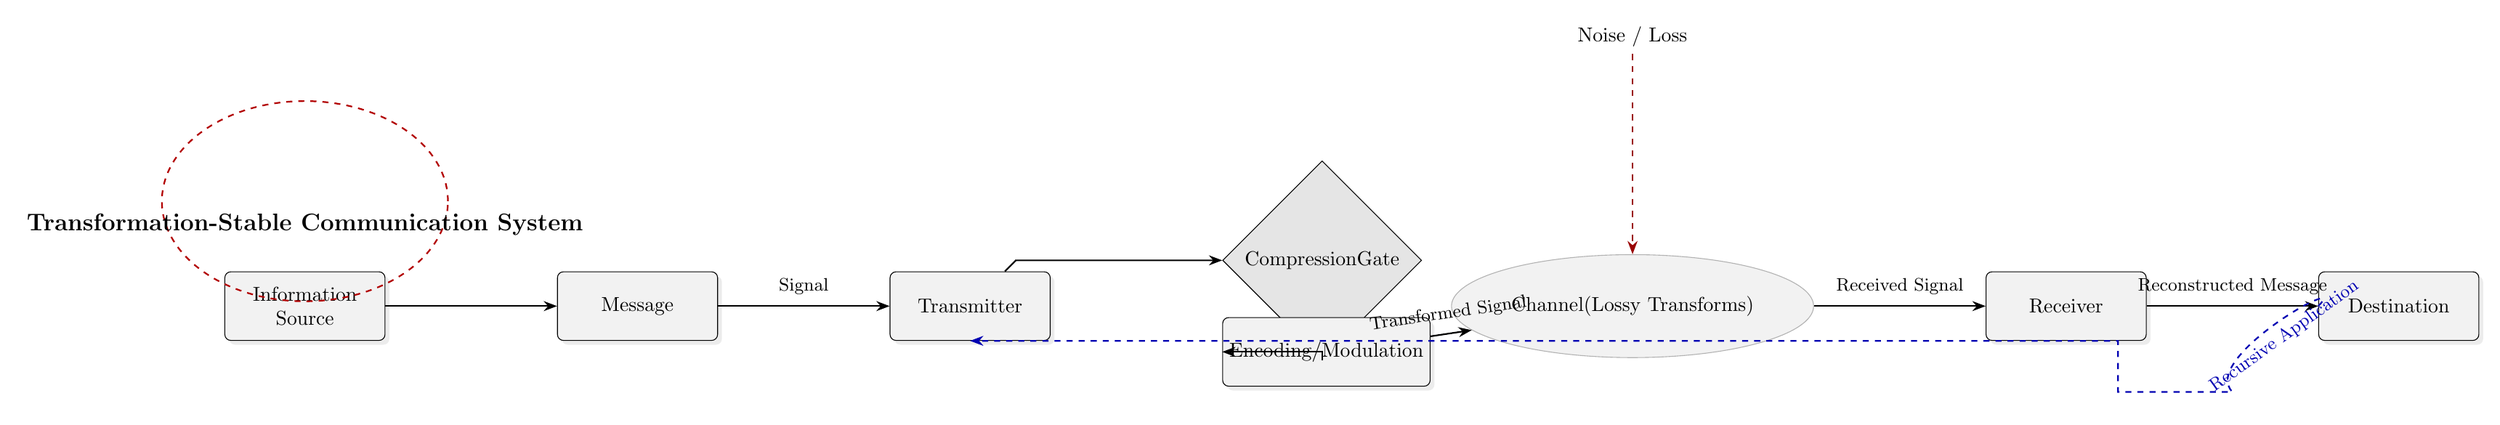
\begin{tikzpicture}[
  >=Stealth,
  node distance=2.5cm and 3cm,
  block/.style={draw, rectangle, rounded corners=3pt, minimum height=1.2cm, minimum width=2.8cm, align=center, fill=white!95!black, drop shadow={opacity=0.15}},
  gate/.style={draw, diamond, minimum height=1.0cm, minimum width=1.8cm, fill=gray!20},
  noisecloud/.style={draw, ellipse, minimum width=3cm, minimum height=1.8cm, fill=gray!10, draw=gray!60},
  arrow/.style={-Stealth, thick},
  label/.style={font=\small, midway, sloped, above=2pt}
]

% Nodes (main chain)
\node[block] (source) {Information\\Source};
\node[block, right=of source] (message) {Message};
\node[block, right=of message] (transmitter) {Transmitter};
\node[gate, right=of transmitter, yshift=0.8cm] (compgate) {Compression\\Gate};
\node[block, right=of transmitter, yshift=-0.8cm] (encoder) {Encoding/Modulation};

% Channel with noise
\node[draw=gray!60, ellipse, minimum width=3cm, minimum height=1.8cm, fill=gray!10, right=of transmitter, xshift=4cm] (channel) {Channel\\(Lossy Transforms)};
\node[block, right=of channel] (receiver) {Receiver};
\node[block, right=of receiver] (destination) {Destination};

% Commitment kernel (highlighted invariant)
\node[draw=red!70!black, thick, dashed, ellipse, minimum width=5cm, minimum height=3.5cm, inner sep=8pt,
      label={[red!70!black]above right:Commitment Kernel\\(Invariant Structure)}] at ($(transmitter)!0.5!(receiver)$) (kernel) {};

% Arrows - forward path
\draw[arrow] (source) -- (message);
\draw[arrow] (message) -- node[label] {Signal} (transmitter);
\draw[arrow] (transmitter) -- ++(0.8,0.8) |- (compgate);
\draw[arrow] (compgate) |- (encoder);
\draw[arrow] (encoder) -- node[label] {Transformed Signal} (channel);
\draw[arrow] (channel) -- node[label] {Received Signal} (receiver);
\draw[arrow] (receiver) -- node[label] {Reconstructed Message} (destination);

% Noise source
\node[above=of channel, yshift=1cm] (noiseSrc) {Noise / Loss};
\draw[arrow, red!60!black, dashed] (noiseSrc) -- (channel);

% Recursive feedback loop (your extension)
\draw[arrow, blue!70!black, dashed, bend right=30] (destination.west) to[out=180,in=270] 
  node[midway, below, sloped, font=\small, blue!70!black] {Recursive Application} 
  ++(-1.5,-1.5) -- ++(-2,0) |- (transmitter.south);

% Optional: label the whole chain
\node[above=0.5cm of source, font=\large\bfseries] {Transformation-Stable Communication System};

\end{tikzpicture}

\end{document}
